\section{Experimental setup and measurement principles}
\subsection{Measurement of relaxation times and chemical shift}
In the first part of the experiment the spin-lattice relaxation time $T_1$ and the spin-spin relaxation time $T_2$ are measured. The spin-spin relaxation time is measured by the spin echo (compare section \ref{sec:1}) as well as by the Carr-Purcell method (compare section \ref{sec:2}). The chemical shift of protons is measured in the following and used to identify five different substances. These measurements are carried out with a Bruker minispec p20, it consists of a Minispec p20 Electronic Unit used signal generation and of a Minispec p20 magnet with a static magnetic field $B_0$. The magnet is shielded by Styrofoam for minimal termperature variation when in use. One can now generate a magnetization $M_{\perp}$ perpendicular or  $M_{\parallel}$ antiparallel to $\vec{B}$ by applying a high frequency pulse $\omega_{HF}$ via the electronic unit to the ground state magnetization $\vec{M}$. We can now rotate the macroscopic magnetization by an angle $\alpha = \gamma_I B_1 \Delta t$ by applying a sinusoidal voltage of given frequency $\omega _{HF}$ for a given time duration $\Delta t$ to a coil oriented perpendicular to the static magnetic field $B_0$. This results in a solenoidal magnetic field $\vec{B}_1$ which is longitudinally polarized in a parallel way with respect to the orientation of the coil. The rotated macroscopic magnetization now precesses around the $B_0$ magnetic field. This in turn induces a voltage into the same coil, which then again represents our measurement signal, which is a mixed signal partially consisting of the so-called working frequency. It is the difference $\nu_{work}=\omega_{HF} - \omega_{Larmor}$ and it has to be calibrated to a value of around $1 kHz$ by varying the Larmor frequency via varying the static magnetic field. The optimal Larmor frequency can be calculated with $\omega_{HF} = 19.8 \mathrm{MHz}$ to be $\omega_{Larmor} = 19.799 \mathrm{MHz}$. The working frequency varied during the measurement by $\pm 50 \mathrm{Hz}$ due to variations in the magnetic field. With $\omega_{Larmor} = \gamma B_0$ we can therefore assume the magnetic field to vary by $\Delta B_0 \approx 5.2\times10^{-5} T$ whilst the temperature of the apparatus changed by $\Delta T \approx 0.01$ \textcelsius. Thus, the systematic error in the calibrated working frequency due to temperature variations can be estimated to be around $\Delta \nu_{work,sys} = 5 \% \nu_{work}$.\\
One can vary the time duration of the applied voltage in order to rotate the magnetization by an angle $\alpha = 90$ \textdegree, 180 \textdegree \, into its perpendicular or antiparallel component with respect to the orientation of $\vec{B} _0$.\cite{manual}


\subsubsection{Spin echo} 
\label{sec:1} In order to measure the spin-spin relaxation time $T_2$ according to equation \ref{eq:2} one starts with a 90 \textdegree\, pulse in order to create a transverse magnetization in y-direction, such that it will precess around the static magnetic field $B_0$ with a given Larmor frequency $\omega_{Larmor} = \gamma B_0$.
\begin{figure}[h]
	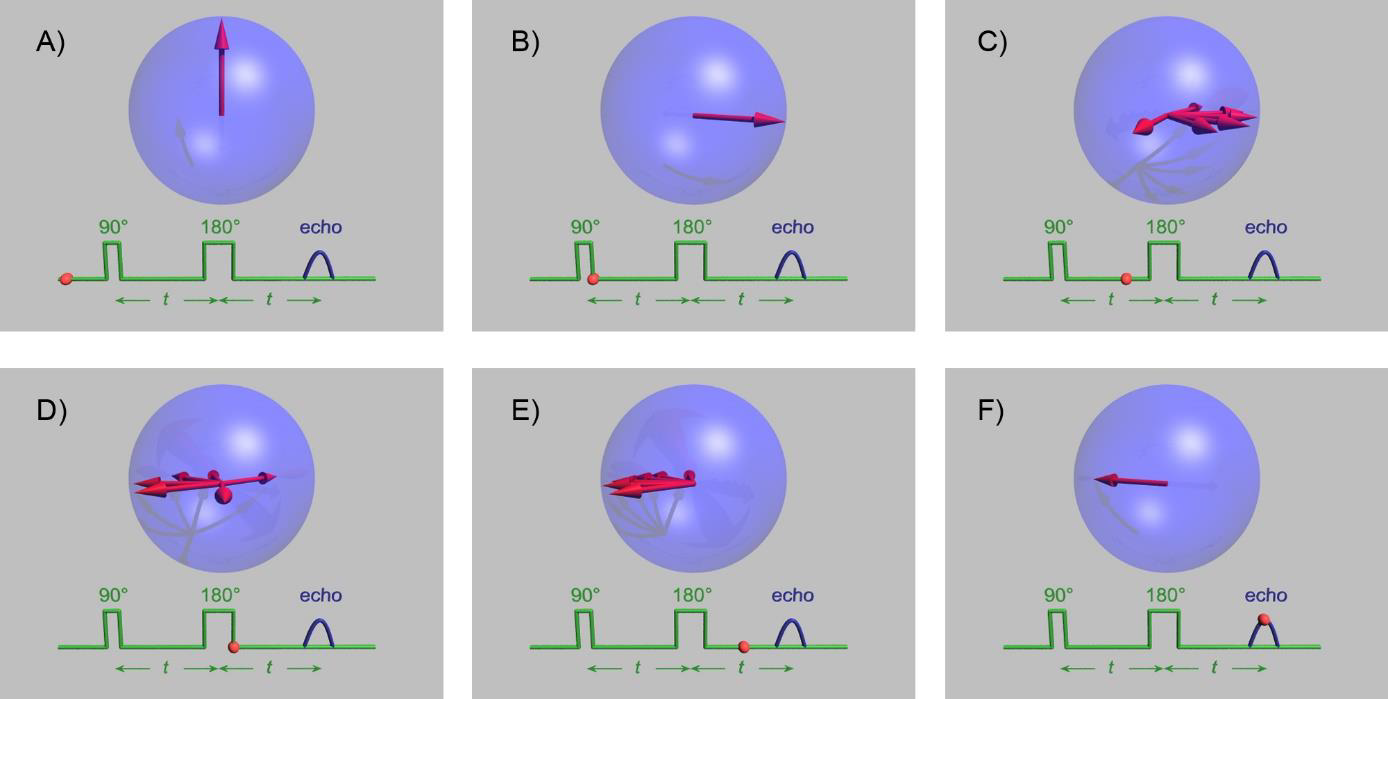
\includegraphics[width=75mm
	]{Spinecho}
	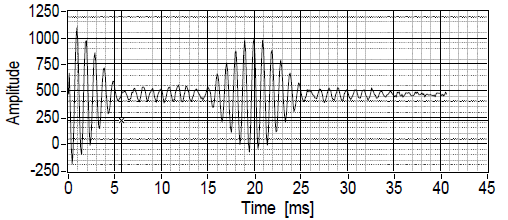
\includegraphics[width=75mm]{Spinecho2}
	\centering
	\caption{\itshape From left to right: Spin echo method \cite{Spinecho}, output signal \cite{manual}}
	\label{fig:1}
\end{figure}
\newpage
\noindent
 Protons at different positions in the probe will now precess with different Larmor frequencies due to the non-linearity of the field, thus phase difference between the protons will develop.
One can now revert the phases of the spins with a 180\textdegree\, pulse in order to guarantee all protons of given phases to coherently align after a given time interval of two times the so-called spin-echo time $\tau$. The induced signal then again represents the relaxation time for the transverse magnetization, which is dominantly caused by spin-spin interactions, thus $T_2$. \cite{manual} \cite{MRI}

 

\subsubsection{Carr-Purcell sequence}
\label{sec:2}
One only achieves approximate alignment of the magnetic dipole moments after $2 \tau$ for long spin echo times due to molecular diffusion happening before the 180 \textdegree\, pulse can be applied. The Carr-Purcell sequence minimizes the effects of molecular diffusion and field inhomogeneities by starting the sequence with a 90 \textdegree\, pulse followed up by a 180 \textdegree\, pulse to ensure phase coherence of the system after $t=2\tau$. One now applies further 180 \textdegree\, pulses for every odd multiple of $\tau$ in order to guarantee phase coherence for every even multiple of $\tau$.
\begin{figure}[h]
	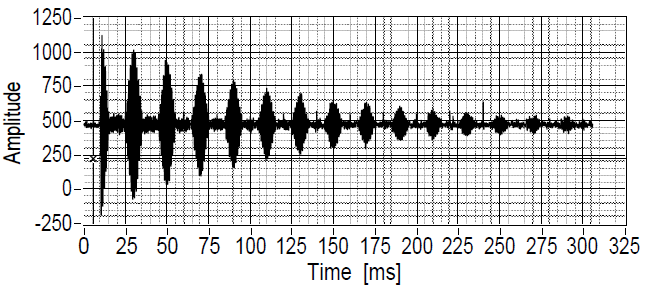
\includegraphics[width=120mm]{CarrPurcell}
	\centering
	\caption{\itshape Carr-Purcell sequence \cite{manual}}
	\label{fig:2}
\end{figure} 
\noindent
A measurement of the spin-spin relaxation time by the Carr-Purcell method hence yields a value which is closer to the true value of the system as compared to the measurement with the spin echo method.\cite{manual}
\label{sec:5}

\subsubsection{Measurement of spin-lattice relaxation $T_1$}

One produces a magnetization antiparallel to the static magnetic field by starting the measurement with the generation of a 180 \textdegree\, pulse. By following this up with a 90 \textdegree\, pulse one measures a signal which represents the current longitudinal magnetization, which is due to spin-lattice interactions and can therefore be used to measure $T_1$.\cite{manual}
\begin{figure}[h]
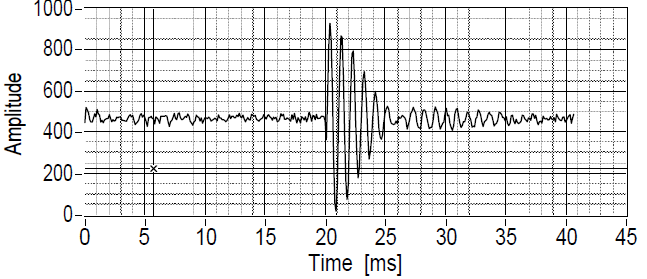
\includegraphics[width=100mm]{T_1}
\centering
\caption{\itshape Pulse sequence 180 \textdegree-90 \textdegree with $\tau$ = 20ms \cite{manual}}
\label{fig:3}
\end{figure}
\subsection{Imaging with NMR}
The imaging measurements are made with the Bruker NMR analyzer mq7.5, where the gradient fields where applied via a system of Helmholtz coils. Nuclear Magnetic Resonance techniques are used for imaging measurements in one and two dimensions. The flow of oil in sand is measured as a time dependent process in one dimension. Two dimensional measurements are carried out to map the inner volume of substances which contain oil or water. The measurement principle of this apparatus is described within section \ref{sec:3}.\cite{manual}
